\section{Gebräuchliche Realisierung von OTA's}
Ein einstufiger OTA wird bereits durch die Differenzstufe realisiert. Dies ist jedoch nicht praktisch da die Last am
Ausgang die Symmetrie der Differenzstufe stört.
Schaltungen siehe Abbildung \ref{fig:otas}!
\begin{figure}[htp]
\begin{center}
	\begin{subfigure}[b]{8cm}
		\centering
		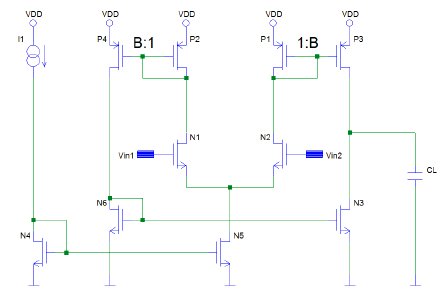
\includegraphics[width=7cm]{images/SymetrischerOTA.png}
		\caption{Symmetrischer OTA}
	\end{subfigure}
	\begin{subfigure}[b]{8cm}
		\centering
		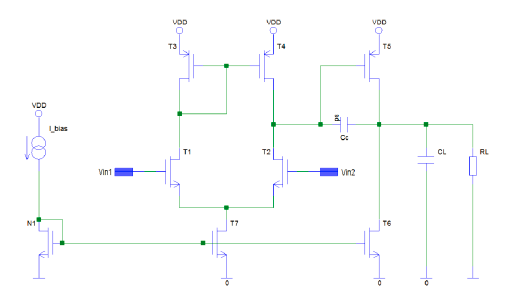
\includegraphics[width=7cm]{images/millerOTA.png}
		\caption{Miller OTA}
	\end{subfigure}
	\caption{Gebräuchliche Realisierungen von OTA's}
	\label{fig:otas}
\end{center}
\end{figure}

\textbf{Verstärkungen:} \\
\begin{tabular}{lll}
	Symmetrischer OTA:	& & $a_v = B \cdot g_{m_{N1}} \cdot (r_{DS_{N3}} || r_{DS_{P3}})$ \\
	Miller OTA:			& & $a_v = a_{v1} \cdot a_{v2} = g_{m1}(r_{DS2} || r_{DS4}) \cdot g_{m5}(r_{DS5} || r_{DS6} || R_L)$
\end{tabular}
